\documentclass[tikz,border=4mm]{standalone}
\usepackage[T1]{fontenc}
\usepackage{lmodern}
\usetikzlibrary{arrows.meta,positioning,calc}
\begin{document}
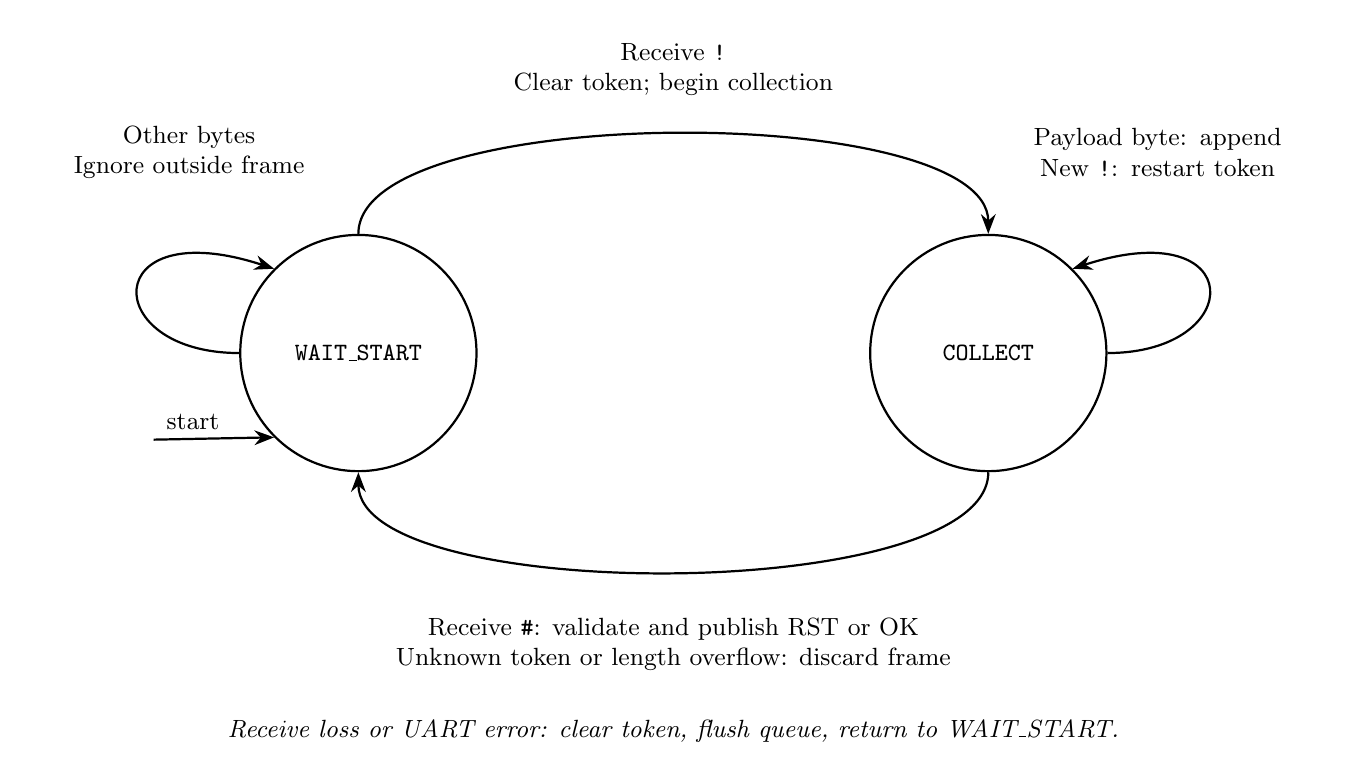
\begin{tikzpicture}[
 font=\small,
 state/.style={circle,draw,thick,minimum size=30mm,align=center,inner sep=1mm,font=\small\bfseries},
 labelbox/.style={align=center,font=\small,inner sep=2mm,fill=white},
 flow/.style={-{Stealth[length=2.5mm]},thick},
 block/.style={draw,rounded corners=2mm,thick,align=center,text width=39mm,minimum height=20mm,inner sep=3mm}]

\node[state] (idle) at (-4,0) {\texttt{WAIT\_START}};
\node[state] (collect) at (4,0) {\texttt{COLLECT}};
\draw[flow] (-6.6,-1.1) -- (idle.south west);
\node[font=\small,above] at (-6.1,-1.1) {start};
\draw[flow] (idle.north) .. controls (-4,3.2) and (4,3.2) .. (collect.north);
\node[labelbox] at (0,3.6) {Receive \texttt{!}\\Clear token; begin collection};
\draw[flow] (collect.south) .. controls (4,-3.2) and (-4,-3.2) .. (idle.south);
\node[labelbox] at (0,-3.7) {Receive \texttt{\#}: validate and publish RST or OK\\Unknown token or length overflow: discard frame};
\draw[flow] (idle.west) .. controls (-7.3,0) and (-7.3,1.8) .. (idle.north west);
\node[labelbox,text width=37mm] at (-6.15,2.55) {Other bytes\\Ignore outside frame};
\draw[flow] (collect.east) .. controls (7.3,0) and (7.3,1.8) .. (collect.north east);
\node[labelbox,text width=37mm] at (6.15,2.55) {Payload byte: append\\New \texttt{!}: restart token};
\node[align=center,font=\small\itshape] at (0,-4.8) {Receive loss or UART error: clear token, flush queue, return to WAIT\_START.};

\end{tikzpicture}
\end{document}
